\documentclass[9pt,table,xcolor=dvipsnames]{beamer}% {{{
\setbeamercovered{invisible}
 %  \documentclass[compress,trans,9pt,table]{beamer}
% \documentclass[compress,9pt,usenames,dvipsnames]{beamer}
% \documentclass[9pt]{beamer}
% \usepackage[utf8]{inputenc}
\setbeamercovered{dynamic}
\usepackage{etex}
\usepackage{multirow}
\usepackage{amsmath}
\usepackage{graphicx,url,psfrag}
\usepackage{tikz}
\usetikzlibrary{
  arrows,
  arrows.meta,
  calc,
  decorations.fractals,
  decorations.pathreplacing,
  graphs,
  mindmap,
  positioning,
  shapes.geometric,
  through,shapes,patterns,
  trees,
  positioning
  }
\usepackage{smartdiagram}
\usesmartdiagramlibrary{additions}
\usepackage[center]{subfigure}
\usepackage{enumerate}
\usepackage[makeroom]{cancel}
\usepackage{mathtools}
\newcommand{\Crossme}[1]{\!\!
\tikz [black,x=1.1em,y=1.1em,line width=.4ex]
\draw (-0.5,-0.5) -- (0,0) node {\footnotesize #1} -- (0.5,0.5) (0.5,-0.5) -- (-0.5,0.5);}%
\newcommand{\Checkme}[1]{\!\!
\tikz [x=1.1em,y=1.1em,line width=.4ex]
\draw [black] (0,0.7) -- (0.3,0) --(0.9,1.0) (0.5,0.5) node {\footnotesize #1};}
\beamerdefaultoverlayspecification{<+-| alert@+>} %(this will show line by line)
\beamerdefaultoverlayspecification{<+->} %(this will show line by
\usepackage{arydshln}
% Smiley face\Smiley{} \Frowny{}
\usepackage{marvosym}

% -------------------------------------------------
%  Set directory for figs
% -------------------------------------------------
\usepackage{grffile}
\graphicspath{{../2016-11-29-McGill/figs/}}

% -------------------------------------------------
%  Define colors
% -------------------------------------------------
% Darkmode
\usepackage{dbt}
% \newcommand{\myref}[1]{\small {\em #1}}
% \def\excolor{brown}
\usepackage{color}
\usepackage{xcolor}

\usepackage{makecell}
\usepackage{tabstackengine}
\renewcommand\theadalign{bc}
\renewcommand\theadfont{\bfseries}
\renewcommand\theadgape{\Gape[4pt]}
\renewcommand\cellgape{\Gape[4pt]}


% -------------------------------------------------
%  Define short-hand symbols.
% -------------------------------------------------
\newcommand{\B}{\textbf{B}}
\newcommand{\E}{\mathbb{E}}
\newcommand{\D}{\mathbb{D}}
\newcommand{\W}{\dot{W}}
\newcommand{\ud}{\ensuremath{\mathrm{d} }}
\newcommand{\Ceil}[1]{\left\lceil #1 \right\rceil}
\newcommand{\Floor}[1]{\left\lfloor #1 \right\rfloor}
\newcommand{\sgn}{\text{sgn}}
\newcommand{\Lad}{\text{L}_{\text{ad}}^2}
\newcommand{\SI}[1]{\mathcal{I}\left[#1 \right]}
\newcommand{\SIB}[2]{\mathcal{I}_{#2}\left[#1 \right]}
\newcommand{\Indt}[1]{1_{\left\{#1 \right\} }}
\newcommand{\LadInPrd}[1]{\left\langle #1 \right\rangle_{\text{L}_\text{ad}^2}}
\newcommand{\LadNorm}[1]{\left|\left|  #1 \right|\right|_{\text{L}_\text{ad}^2}}
\newcommand{\Norm}[1]{\left|\left|  #1   \right|\right|}
\newcommand{\Ito}{It\^{o} }
\newcommand{\Itos}{It\^{o}'s }
\newcommand{\spt}[1]{\text{supp}\left(#1\right)}
\newcommand{\InPrd}[1]{\left\langle #1 \right\rangle}
\newcommand{\mr}{\textbf{r}}
\newcommand{\Ei}{\text{Ei}}
\newcommand{\arctanh}{\operatorname{arctanh}}
\newcommand{\ind}[1]{\mathbb{I}_{\left\{ {#1} \right\} }}


\DeclareMathOperator{\esssup}{\ensuremath{ess\,sup}}

\newcommand{\steps}[1]{\vskip 0.3cm \textbf{#1}}
\newcommand{\calB}{\mathcal{B}}
\newcommand{\calC}{\mathcal{C}}
\newcommand{\calD}{\mathcal{D}}
\newcommand{\calE}{\mathcal{E}}
\newcommand{\calF}{\mathcal{F}}
\newcommand{\calG}{\mathcal{G}}
\newcommand{\calK}{\mathcal{K}}
\newcommand{\calH}{\mathcal{H}}
\newcommand{\calI}{\mathcal{I}}
\newcommand{\calL}{\mathcal{L}}
\newcommand{\calM}{\mathcal{M}}
\newcommand{\calN}{\mathcal{N}}
\newcommand{\calO}{\mathcal{O}}
\newcommand{\calT}{\mathcal{T}}
\newcommand{\calP}{\mathcal{P}}
\newcommand{\calR}{\mathcal{R}}
\newcommand{\calS}{\mathcal{S}}
\newcommand{\calV}{\mathcal{V}}
\newcommand{\bbC}{\mathbb{C}}
\newcommand{\bbF}{\mathbb{F}}
\newcommand{\bbN}{\mathbb{N}}
\newcommand{\bbP}{\mathbb{P}}
\newcommand{\bbZ}{\mathbb{Z}}
\newcommand{\myVec}[1]{\overrightarrow{#1}}
\newcommand{\sincos}{\begin{array}{c} \cos \\ \sin \end{array}\!\!}
\newcommand{\CvBc}[1]{\left\{\:#1\:\right\}}
\newcommand*{\one}{{ {\rm 1\mkern-1.5mu}\!{\rm I} }}
\newcommand{\Lip}{\text{Lip}}

\newcommand{\bH}{\ensuremath{\mathrm{H} }}
\newcommand{\Ai}{\ensuremath{\mathrm{Ai} }}

\newcommand{\R}{\mathbb{R}}
\newcommand{\myEnd}{\hfill$\square$}
\newcommand{\ds}{\displaystyle}
\newcommand{\Shi}{\text{Shi}}
\newcommand{\Chi}{\text{Chi}}
\newcommand{\Erf}{\ensuremath{\mathrm{erf} }}
\newcommand{\Erfc}{\ensuremath{\mathrm{erfc} }}
\newcommand{\He}{\ensuremath{\mathrm{He} }}
\newcommand{\Res}{\ensuremath{\mathrm{Res} }}

\newcommand{\mySeparateLine}{
\begin{center}
\makebox[\linewidth]{\rule{0.6\paperwidth}{0.4pt}}
\end{center}}

% The following is to increase the gap in underbrace.
% Followed by https://tex.stackexchange.com/questions/13843/vertical-spacing-with-underbrace-command/13864
\newcommand*\mystrut[1]{\vrule width0pt height0pt depth#1\relax}

% % % Define danger sign
\newcommand*{\TakeFourierOrnament}[1]{{%
\fontencoding{U}\fontfamily{futs}\selectfont\char#1}}
\newcommand*{\danger}{\TakeFourierOrnament{66}}

\theoremstyle{definition}
% \newtheorem{definition}[theorem]{Definition}
% \newtheorem{hypothesis}[theorem]{Hypothesis}
\newtheorem{assumption}[theorem]{Assumption}

\theoremstyle{plain}
% \newtheorem{theorem}{Theorem}
% \newtheorem{corollary}[theorem]{Corollary}
% \newtheorem{lemma}[theorem]{Lemma}
\newtheorem{proposition}[theorem]{Proposition}

\mode<presentation>
{
%      \usetheme{Warsaw}
%     \usetheme{JuanLesPins}
%  \usetheme{Hannover}
%  \usetheme{Montpellier}
   % \useoutertheme{default}
  % or ...

  \setbeamercovered{transparent}
  % or whatever (possibly just delete it)
 \setbeamertemplate{frametitle}{
  \begin{centering}
    \color{lgtblue!70!black}{\insertframetitle}
    \par
  \end{centering}
  }
}
\usefoottemplate{\hfill \insertframenumber{} / 24}
% \inserttotalframenumber

\usepackage[english]{babel}
% or whatever

% \usepackage[latin1]{inputenc}
% or whatever

\usepackage{times}
\usepackage[T1]{fontenc}
% Or whatever. Note that the encoding and the font should match. If T1
% does not look nice, try deleting the line with the fontenc.

% \DeclareMathOperator{\Lip}{Lip}
\DeclareMathOperator{\lip}{l}
% \DeclareMathOperator{\Vip}{\overline{v}}
% \DeclareMathOperator{\vip}{\underline{v}}
% \DeclareMathOperator{\vv}{v}
% \DeclareMathOperator{\BC}{BC}
% \DeclareMathOperator{\CH}{CD}

\usepackage{pgfpages}
% \setbeameroption{show notes}
% \setbeamertemplate{note page}[plain]
% \setbeameroption{second mode text on second screen=right}
% \setbeameroption{show notes on second screen=right}
%

\AtBeginSection[]
  {
     \begin{frame}<beamer>
     % \frametitle{Plan}
     \tableofcontents[currentsection]
     \end{frame}
  }
% }}}
\title{Sharpening your saw before cutting down the tree
\\ -- Personal development environment (PDE)}% {{{

% \subtitle
% {Research Plan} % (optional)

\author{Le Chen\\
Auburn University
}
% - Use the \inst{?} command only if the authors have different
%   affiliation.
\institute[Auburn University]
{%
% \vspace{3em}
\pgfuseimage{Emory}
 }
 \vfill
% - Use the \inst command only if there are several affiliations.
% - Keep it simple, no one is interested in your street address.

% \date[Talk at Karlsruhe] % (optional)
% {\today }
\date[Columbus]{
  \footnotesize
  Graduate Student Seminar \\[1em]
  Department of Mathematics \& Statistics\\[0.5em]
  Auburn University\\[1em]
  Feb. 15th 2023\\
}

% This is only inserted into the PDF information catalog. Can be left
% out.

% If you have a file called "university-logo-filename.xxx", where xxx
% is a graphic format that can be processed by latex or pdflatex,
% resp., then you can add a logo as follows:

\pgfdeclareimage[height=1.2cm]{Emory}{figs/AU-Black.jpeg}

% Delete this, if you do not want the table of contents to pop up at
% the beginning of each subsection:
% \AtBeginSubsection[]
% {
%   \begin{frame}<beamer>{Outline}
%     \tableofcontents[currentsection,currentsubsection]
%   \end{frame}
% }


% If you wish to uncover everything in a step-wise fashion, uncomment
% the following command:

% \beamerdefaultoverlayspecification{<+->}

\begin{document}
% }}}
\begin{frame}[noframenumbering]
  \titlepage
\end{frame}
% \begin{frame}
%   \tableofcontents
%   % You might wish to add the option [pausesections]
% \end{frame}
\begin{frame}[fragile] % COMENTS
  \bigskip
  \begin{center}
    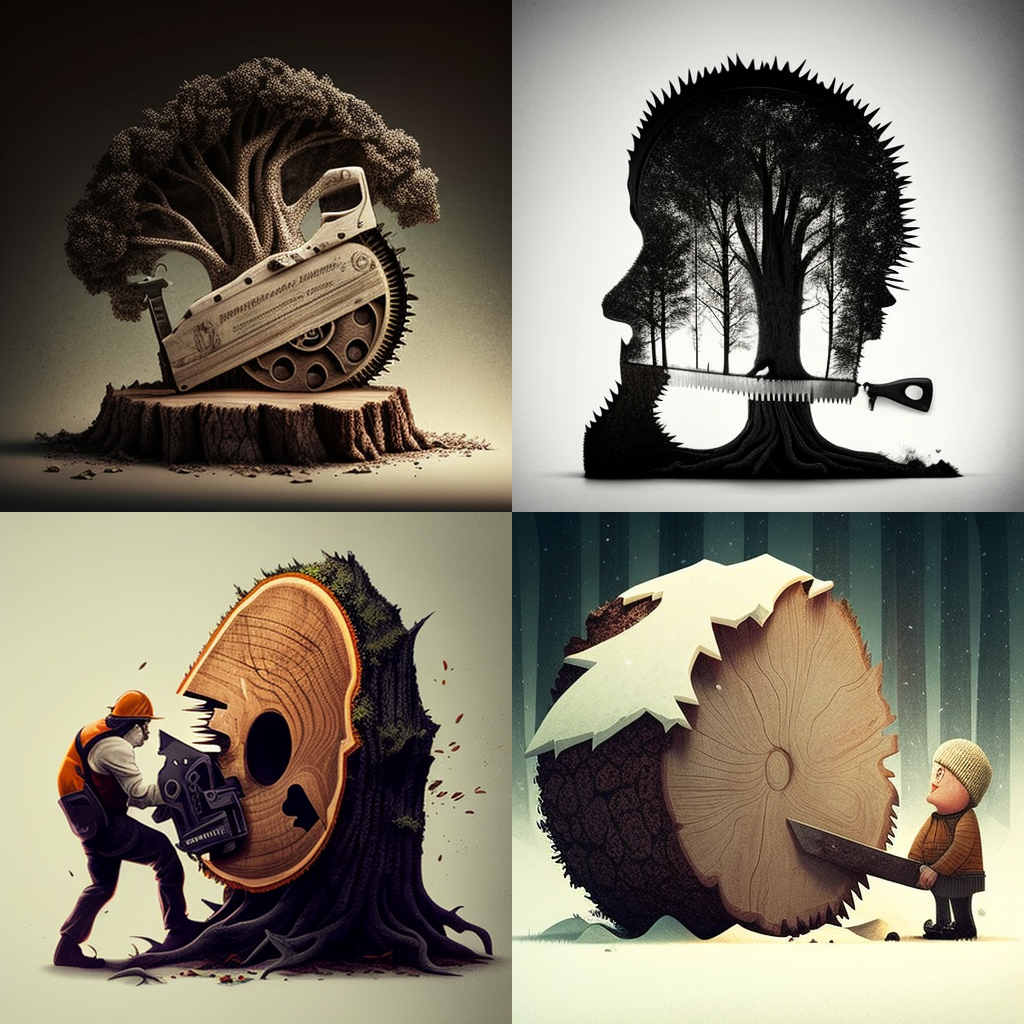
\includegraphics[scale=0.25]{./figs/chenle02_Illustrate_the_idea_If_you_sharpen_the_saw_you_would.png}
  \end{center}
\end{frame}
\section{Introduction to vi/vim/nvim}
\begin{frame}
  \frametitle{What is Vi/Vim?}
  \begin{itemize}
    \item Text editor designed for speed and efficiency
    \item Built-in support for many programming languages and file types
    \item Highly customizable and extensible through plugins and configurations
    \item Available on most platforms (including Linux, macOS, and Windows)
  \end{itemize}
\end{frame}
\begin{frame}
  \frametitle{What is NeoVim?}
  \begin{itemize}
    \item Fork of Vim with many additional features and improvements
    \item Decouples Vim from its legacy architecture to enable easier maintenance and extension
    \item Built-in support for features such as asynchronous plugins, better integration with terminals, and remote plugins
  \end{itemize}
\end{frame}
\begin{frame}
  \frametitle{History of Vim and NeoVim}
  \begin{itemize}
    \item 1976 - vi is created by Bill Joy at UC Berkeley
    \item 1991 - Vim (Vi Improved) is released by Bram Moolenaar
    \item 2014 - NeoVim is forked from Vim by Thiago de Arruda and other developers
    \item 2015 - NeoVim 0.1.0 is released, featuring many new features and improvements over Vim
    \item 2023 - Latest release of Vim is version 8.2, and latest release of NeoVim is version 0.9.0
  \end{itemize}
\end{frame}
\begin{frame}
  \frametitle{Advantages of NeoVim}
  \begin{itemize}
    \item Asynchronous plugins - Plugins can run in the background without blocking the editor
    \item Better terminal integration - Built-in terminal emulator for running shell commands
    % \item Remote plugins - Plugins can run on a different machine and interact with the editor through a message protocol
    \item Simplified configuration - NeoVim uses a Lua-based configuration system that is easier to read and write than Vim's configuration
    \item Improved performance - NeoVim's architecture allows it to be faster and more stable than Vim, especially with large files or complex operations
  \end{itemize}
\end{frame}
\begin{frame}[fragile] % COMENTS
  \frametitle{Editor holy war}
  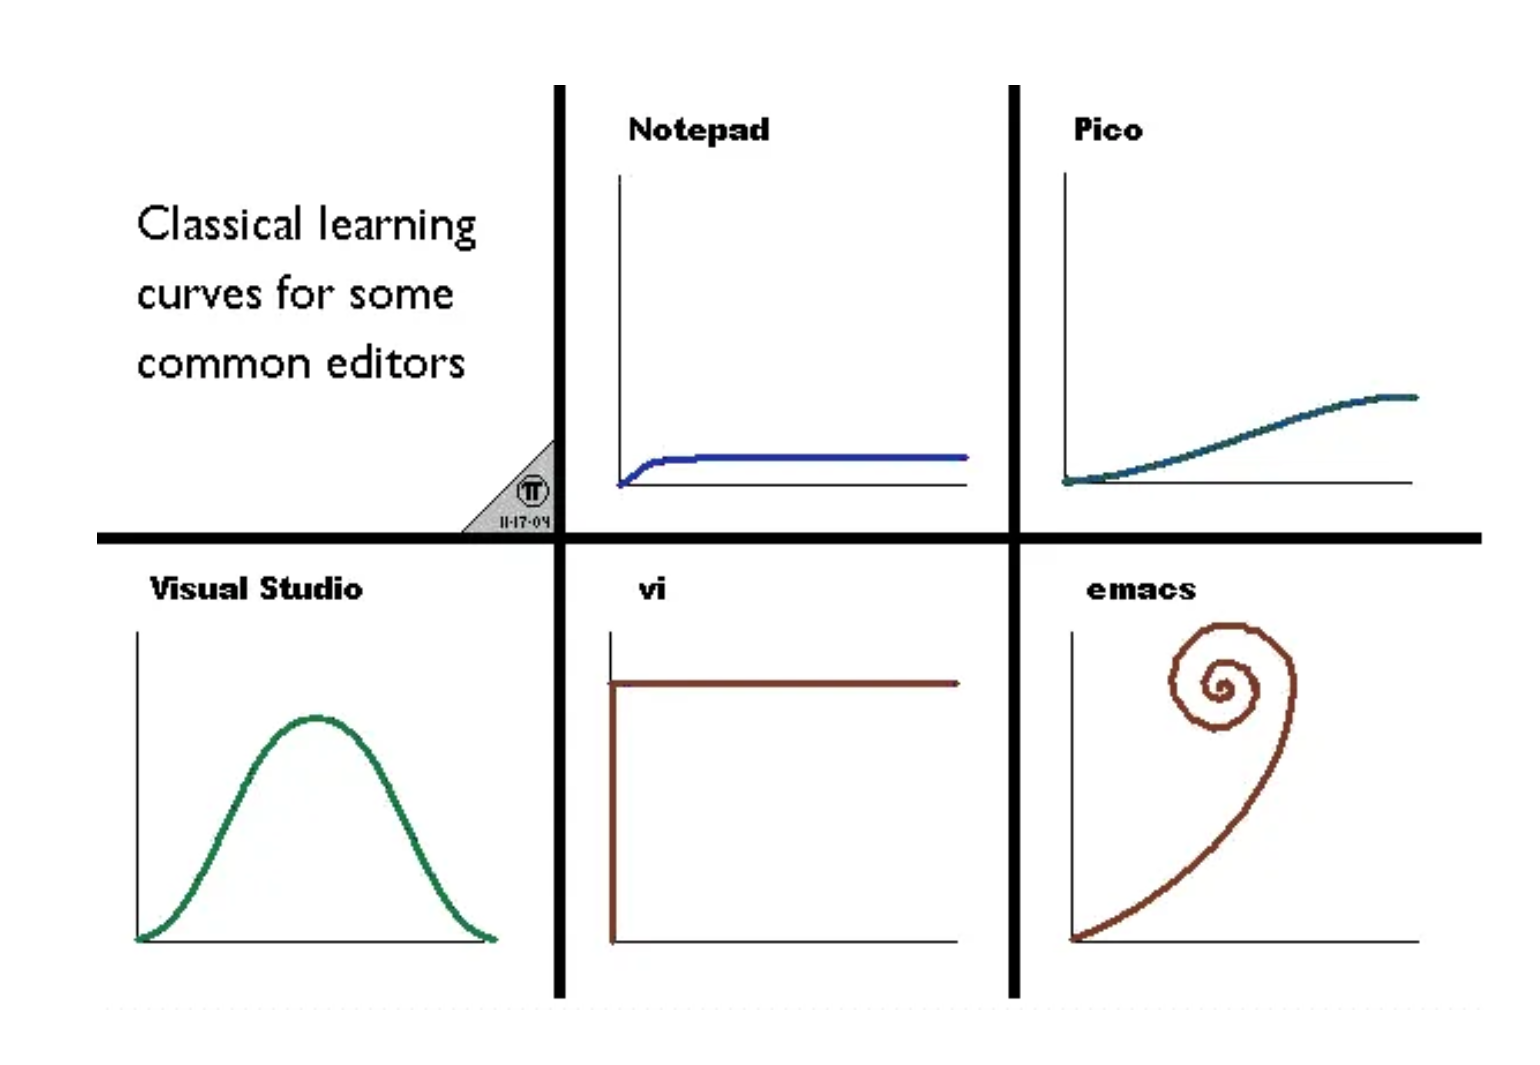
\includegraphics[scale=0.20]{./figs/Learning_Curve.png}\footnote{Image from \url{https://prajwollamichhane11.medium.com/vim-vs-emacs-the-editor-war-b63ecb12ea92}}
\end{frame}
\begin{frame}[fragile,t] % COMENTS
  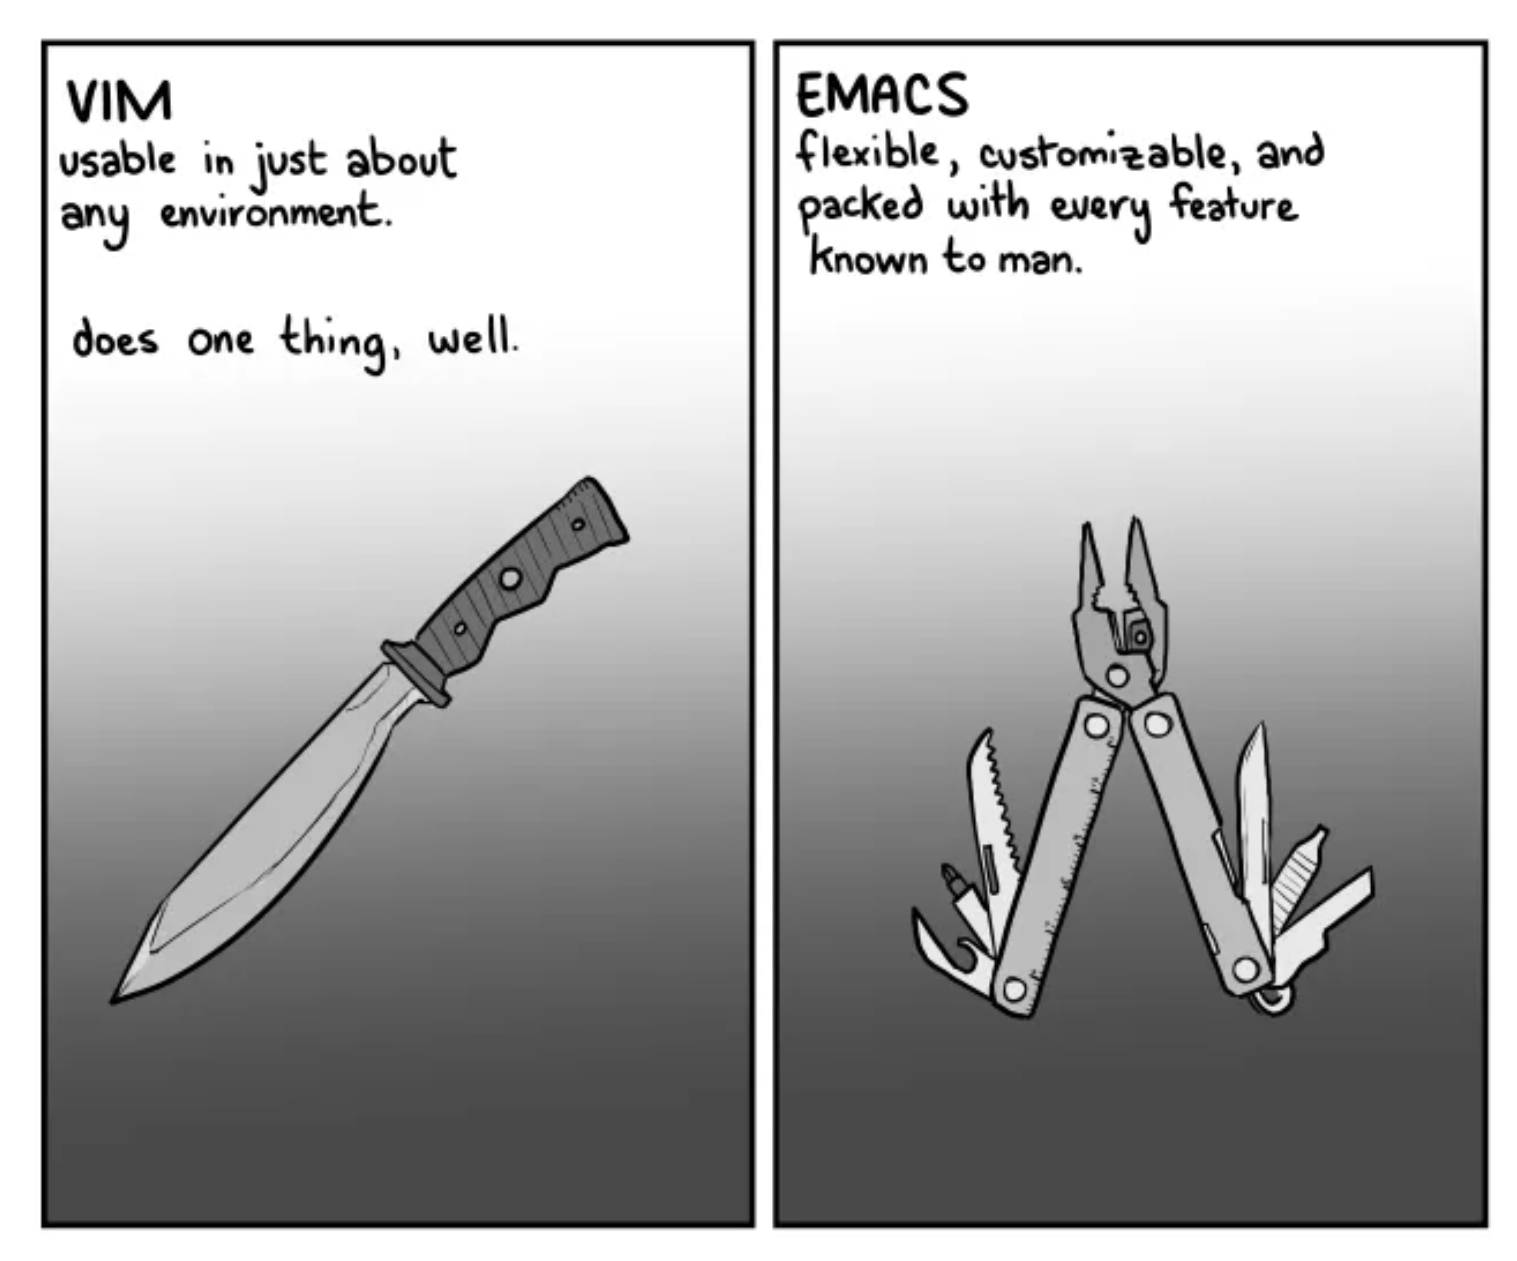
\includegraphics[scale=0.18]{./figs/Vim_vs_Emas.png}
  \footnote{Image from \url{https://prajwollamichhane11.medium.com/vim-vs-emacs-the-editor-war-b63ecb12ea92}}
\end{frame}
\begin{frame}
  \frametitle{Basic Vim Commands}
  \begin{itemize}
    \item Three modes: normal, insert, and visual
    \item Navigation: h, j, k, l, w, b, e, 0, \$, gg, G, f, F, t, T
    \item Editing: i, a, o, I, A, O, r, d, D, y, Y, p, P, u, x
    \item Saving and quitting: :w, :wq, :q, :q!, :w!, :wq!
    \item[]
    \item Text objects in VimTex:
    \item[] \textcolor{magenta}{\bf c} (change), \textcolor{magenta}{\bf v} (visual
      select), \textcolor{magenta}{\bf t} (toggle), \textcolor{magenta}{\bf d} (delete)
    \item[] \textcolor{green}{\bf i} (inside), \textcolor{green}{\bf a} (around),
      \textcolor{green}{\bf s} (surround)
    \item[] e (environment), \$ (inline math), s (sentence), p (paragraph), w (word), W (word)
    \item[]
    \item Macros: q, @
    \item Snippets: tab
    \item[]
    \item Searching and replacing: /, ?, n, N, :s, :s/, g, gc
  \end{itemize}
\end{frame}
\begin{frame}[fragile] % COMENTS
  % Fun video about Vim:

  Interview with a VIM Enthusiast \\ \bigskip

  \url{https://www.youtube.com/watch?v=9n1dtmzqnCU&t=141s}
\end{frame}
\section{Using git/github to track your progress}
\subsection{What is Git?}
\begin{frame}
  \frametitle{What is Git?}
  \begin{itemize}
    \item Distributed version control system
    \item Tracks changes to code over time
    \item Enables collaboration and easy rollback
  \end{itemize}
\end{frame}
\subsection{Basic Git Commands}
\begin{frame}
  \frametitle{Basic Git Commands}
  \begin{itemize}
    \item git init
    \item git add
    \item git commit
    \item git push
    \item git pull
    \item git clone
  \end{itemize}
\end{frame}
\subsection{What is GitHub?}
\begin{frame}
  \frametitle{What is GitHub?}
  \begin{itemize}
    \item Web-based platform for Git repositories
    \item Provides collaboration features (e.g., pull requests)
    \item Includes project management tools (e.g., issues, milestones)
  \end{itemize}
\end{frame}
\subsection{Getting Started with Git and GitHub}
\begin{frame}
  \frametitle{Getting Started with Git and GitHub}
  \begin{itemize}
    \item Install Git on your computer
    \item Create a GitHub account
    \item Create a new repository on GitHub
    \item Clone the repository to your local machine
    \item Add files and commit changes
    \item Push changes to the remote repository
  \end{itemize}
\end{frame}
\subsection{Conclusion}
\begin{frame}
  \frametitle{Conclusion}
  \begin{itemize}
    \item Git and GitHub are powerful tools for managing code and collaborating with others
    \item By using Git and GitHub, you can easily keep track of changes to your code and work more efficiently with others
    \item Practice using Git and GitHub regularly to become proficient in using these tools
  \end{itemize}
\end{frame}
\section{Chatgpt}
\begin{frame}[fragile] % COMENTS
  % \frametitle{What is it good at?}

  \textbf{What is it good at?}

   \begin{enumerate}
     \item Write codes (all languages) -- Work automation.
     \item Write essay, poem, etc. -- for fun.
     \item Revise general purposed text.
   \end{enumerate}

  \vfill

  \textbf{What is it not good at?}

   \begin{enumerate}
     \item Mathematically intensive tasks
     \item Literature review (be really careful)
   \end{enumerate}

\end{frame}

\section{Gallery generated by \textit{Midjourney}}
\begin{frame}[fragile] % COMENTS
  \begin{center}
    \Large
    Some fun images generated by \textit{Midjourney}\\ \bigskip
    for this talk. \bigskip

    Enjoy~!
  \end{center}
\end{frame}
\begin{frame}[fragile,t] % COMENTS
  \frametitle{Illustrate the idea If you sharpen the saw you would...}
  \begin{center}
    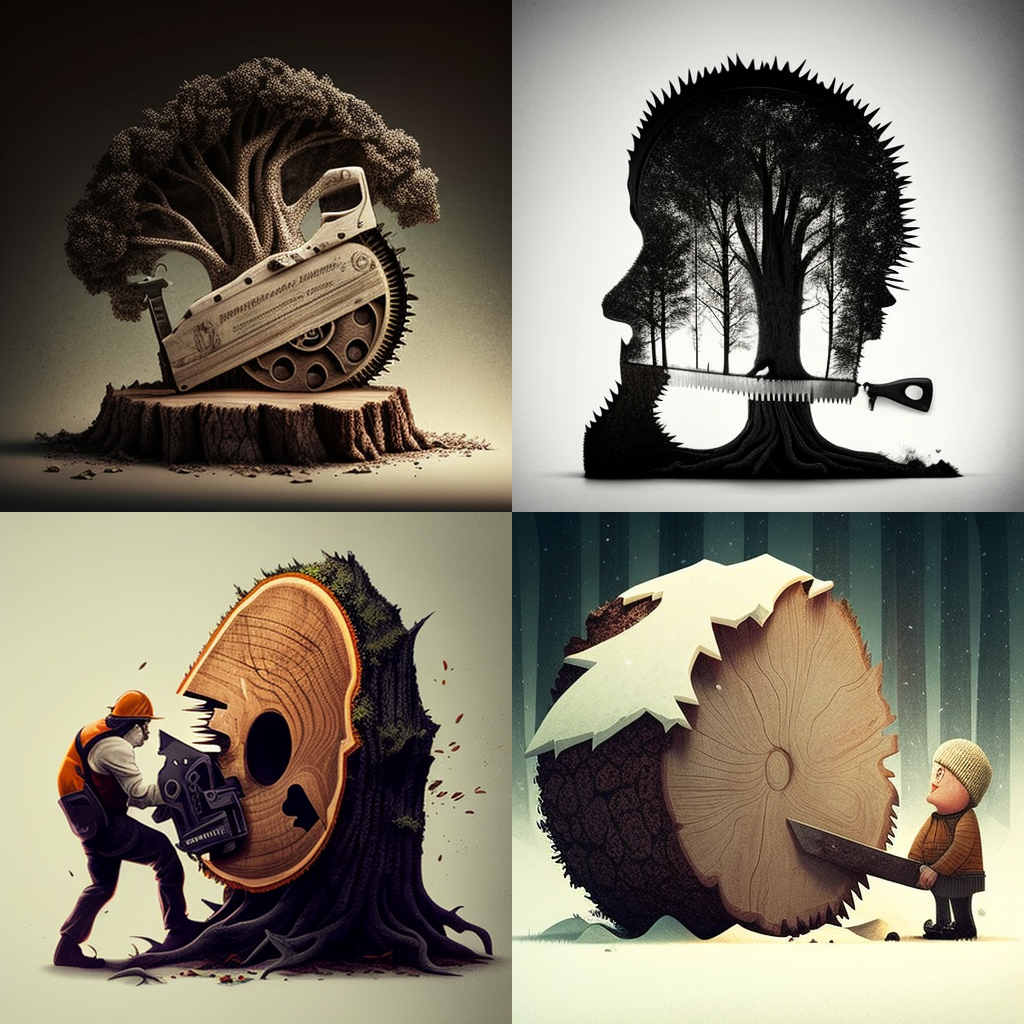
\includegraphics[scale=0.22]{./figs/chenle02_Illustrate_the_idea_If_you_sharpen_the_saw_you_would.png}
  \end{center}
\end{frame}
\begin{frame}[fragile,t] % COMENTS
  \frametitle{Illustrate the idea If you sharpen the saw you would...}
  \begin{center}
    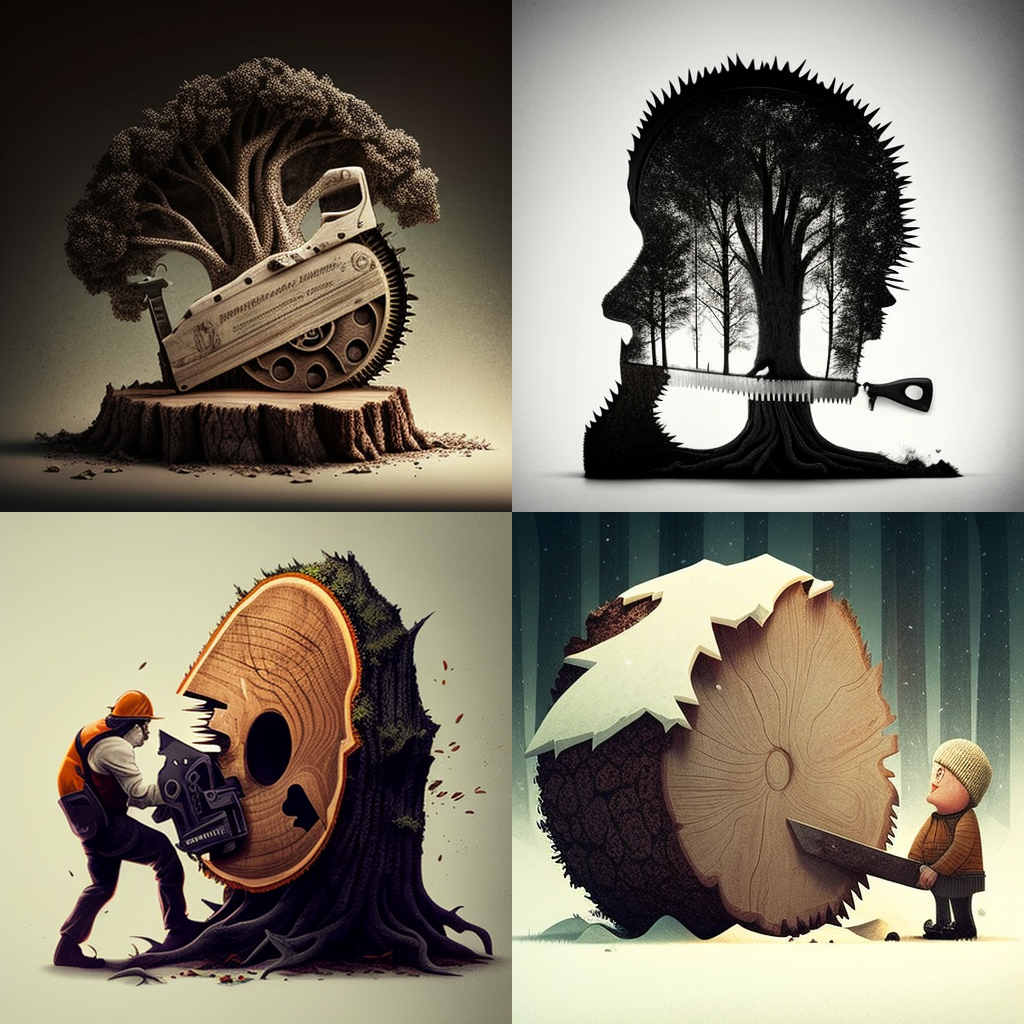
\includegraphics[scale=0.22]{./figs/chenle02_Illustrate_the_idea_If_you_sharpen_the_saw_you_would.png}
  \end{center}
\end{frame}
\begin{frame}[fragile,t] % COMENTS
  \frametitle{Illustrate the idea If you sharpen the saw you can cut...}
  \begin{center}
    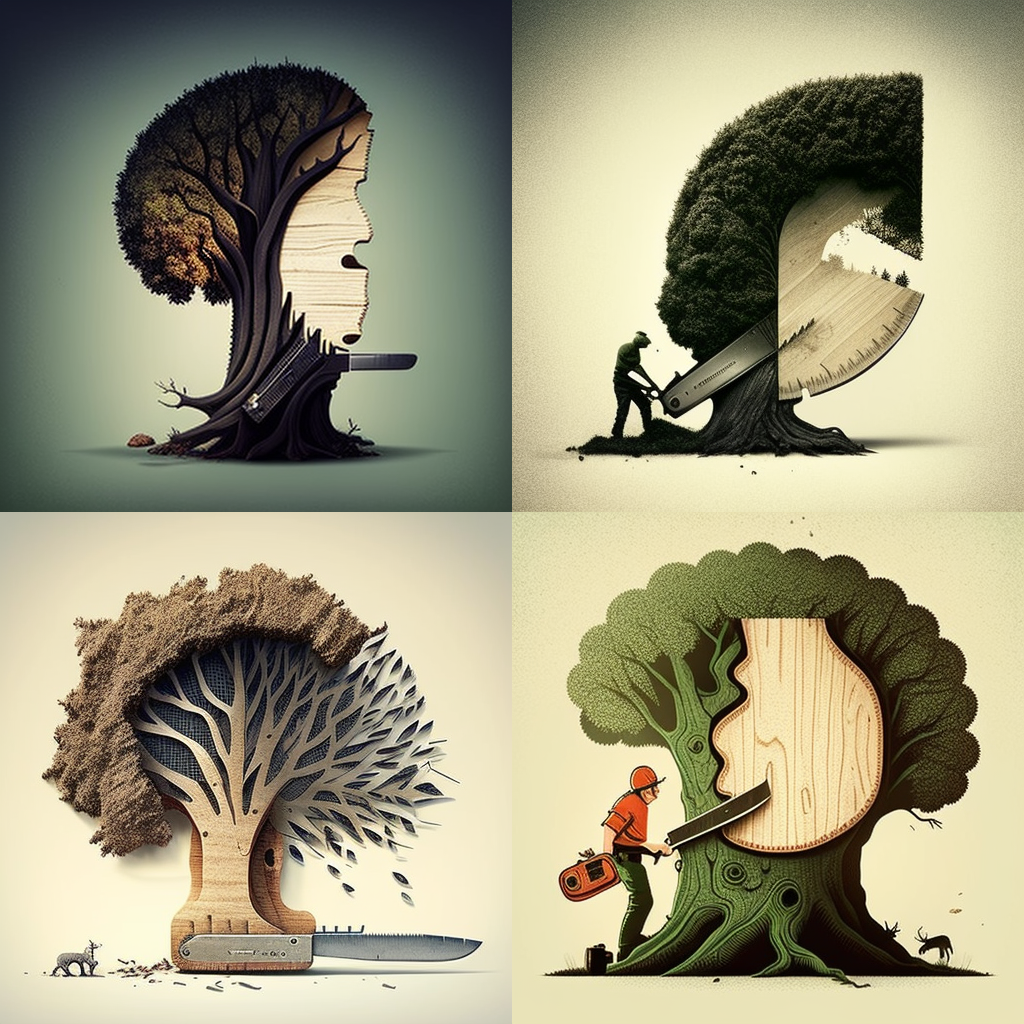
\includegraphics[scale=0.22]{./figs/chenle02_illustrate_the_idea_If_you_sharpen_the_saw_you_can_cut.png}
  \end{center}
\end{frame}
\begin{frame}[fragile,t] % COMENTS
  \frametitle{Two guys are lumbering one with advanced tool doing...}
  \begin{center}
    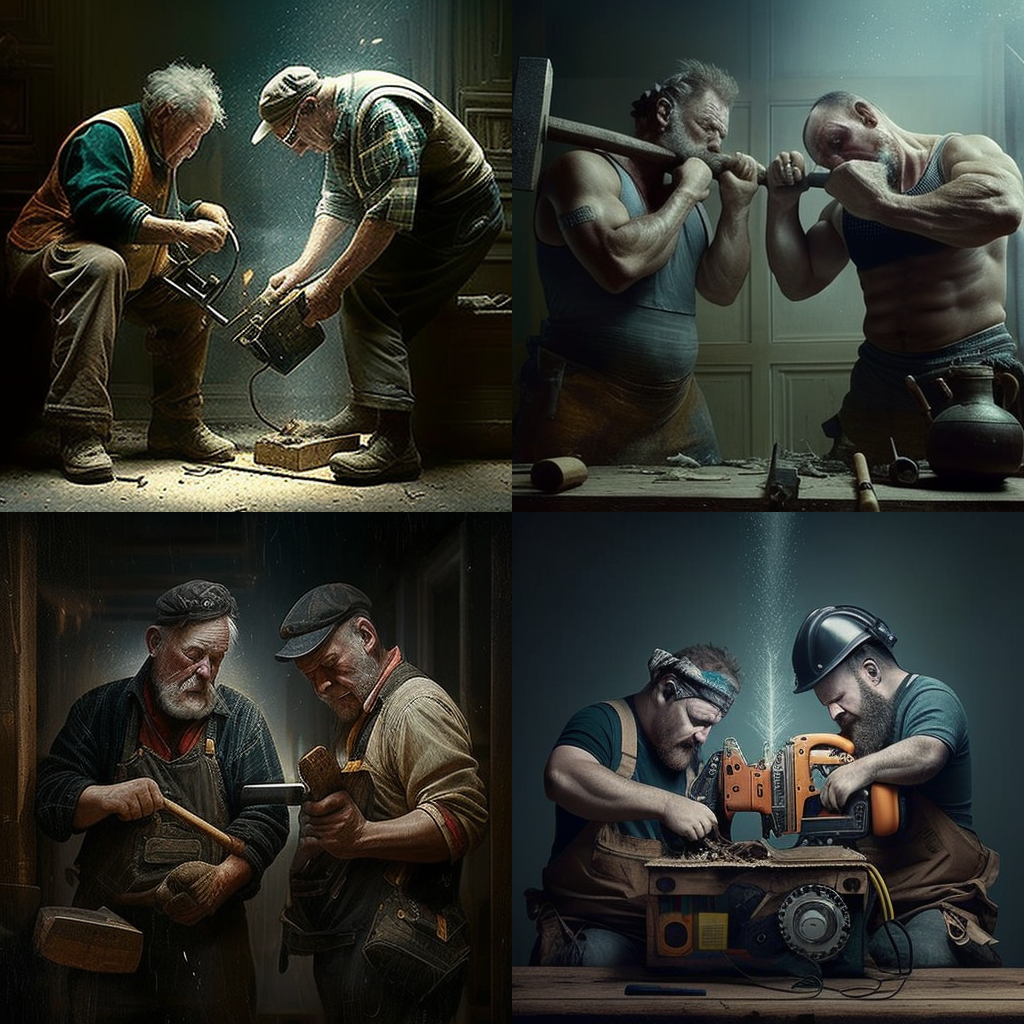
\includegraphics[scale=0.22]{./figs/chenle02_two_guys_are_Lumbering_one_with_advanced_tool_doing_th.png}
  \end{center}
\end{frame}
\begin{frame}[fragile,t] % COMENTS
  \frametitle{Illustrate the idea of Time taken for sharpening...}
  \begin{center}
    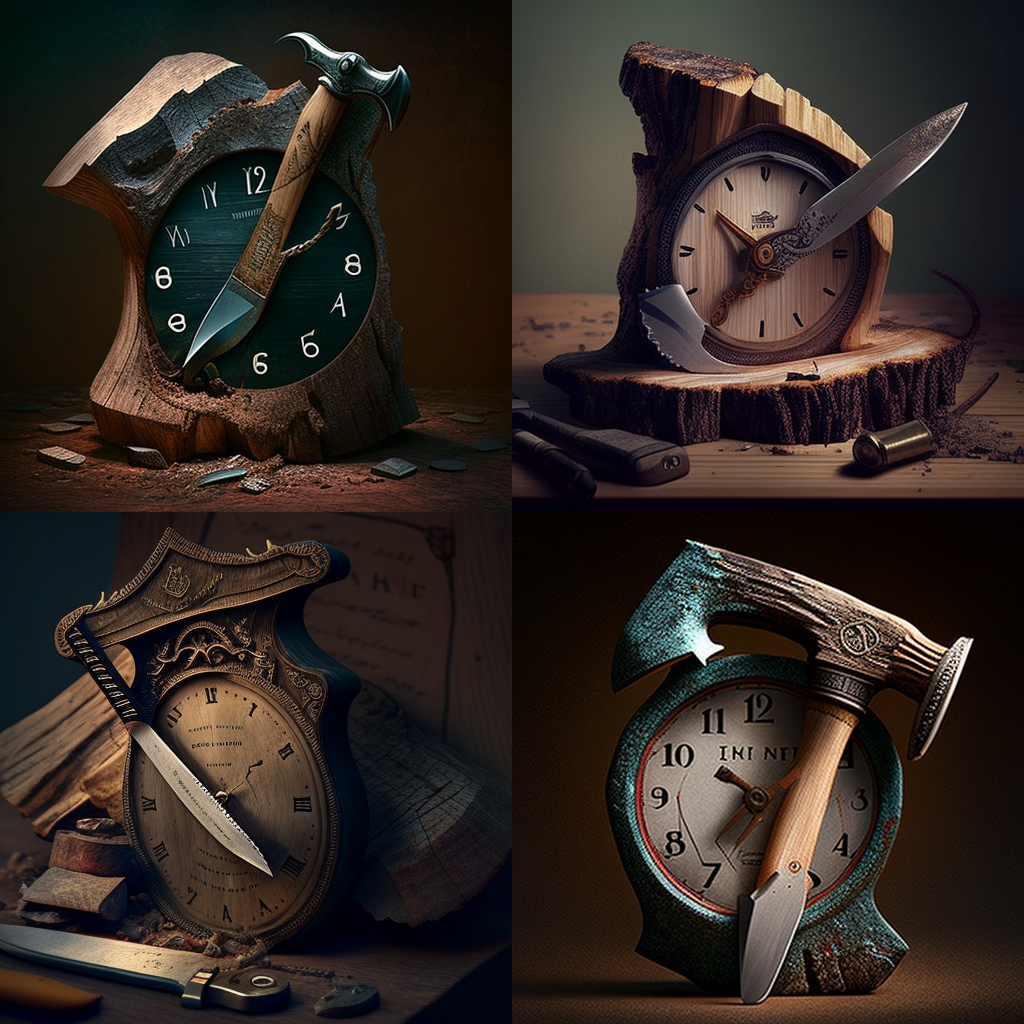
\includegraphics[scale=0.22]{./figs/chenle02_Illustrate_the_idea_of_Time_taken_for_sharpening_the_a.png}
  \end{center}
\end{frame}
\begin{frame}[fragile,t] % COMENTS
  \frametitle{Show sharp tools are superior than dull tools...}
  \begin{center}
    
\includegraphics[scale=0.22]{./figs/chenle02_Show_sharp_tools_are_superior_than_dull_tools_illustra.png}
  \end{center}
\end{frame}
\begin{frame}[fragile,t] % COMENTS
  \frametitle{Illustrate An artisan must first sharpen his tools if...}
  \begin{center}
    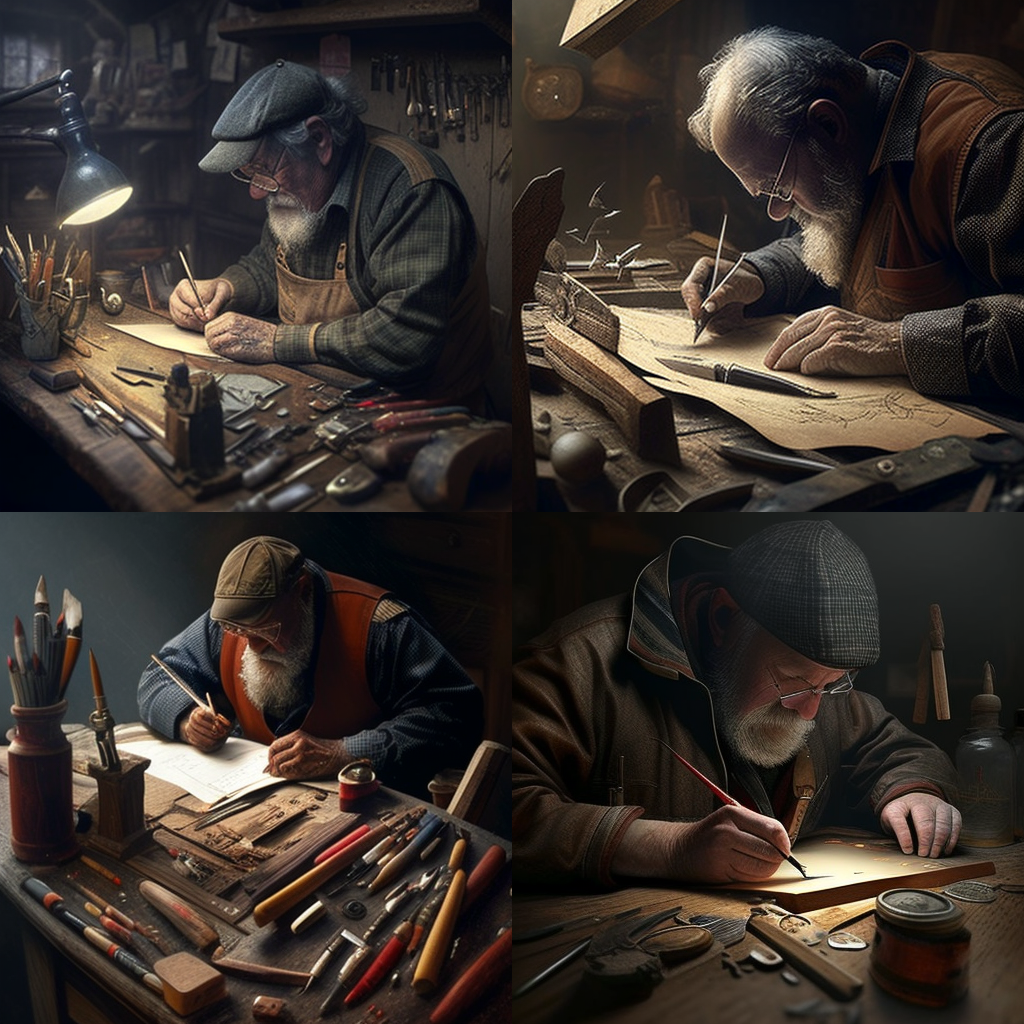
\includegraphics[scale=0.22]{./figs/chenle02_Illustrate_An_artisan_must_first_sharpen_his_tools_if.png}
  \end{center}
\end{frame}
\begin{frame}[fragile,t] % COMENTS
  \frametitle{Chaotic stochastic heat flow on a torus...}
  \begin{center}
    
\includegraphics[scale=0.22]{./figs/chenle02_Chaotic_stochastic_heat_flow_on_a_torus.png}
  \end{center}
\end{frame}
\begin{frame}[fragile,t] % COMENTS
  \frametitle{Law of large numbers and central limit theorem...}
  \begin{center}
    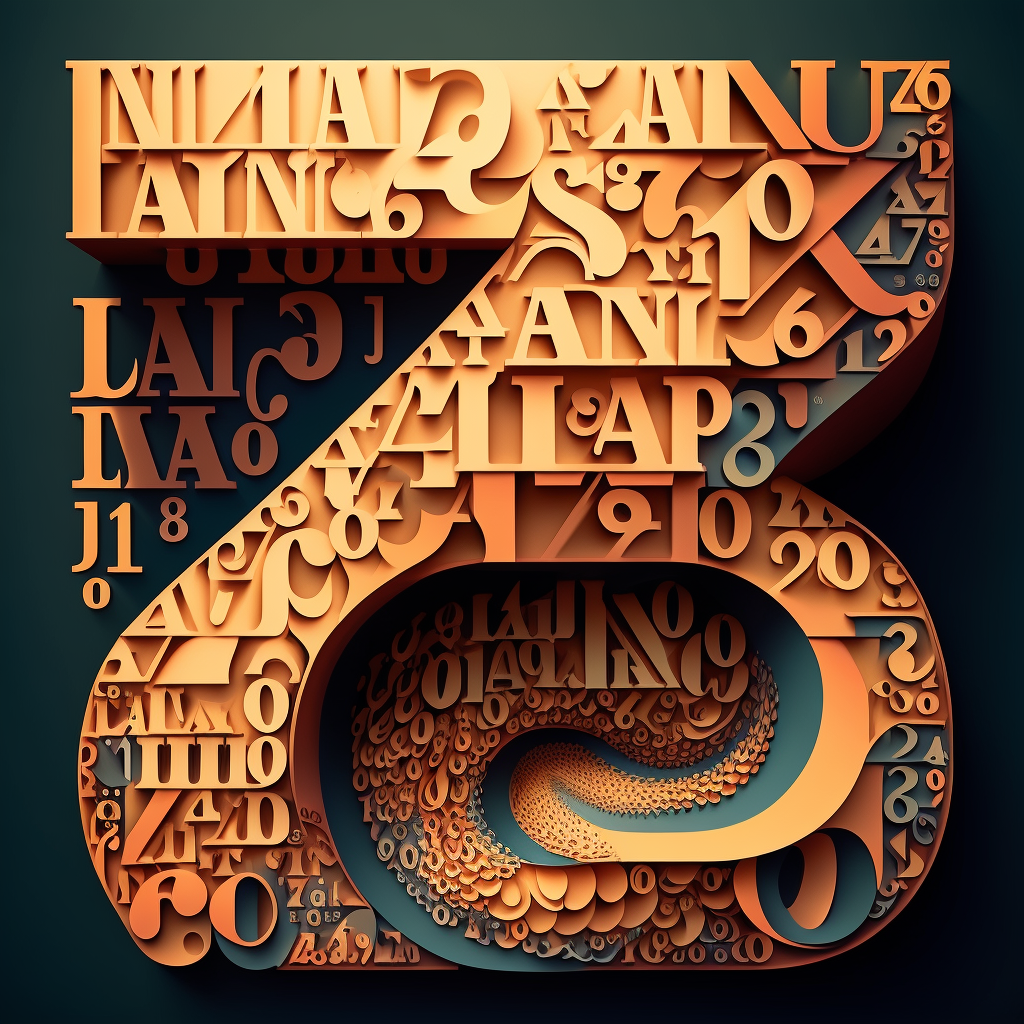
\includegraphics[scale=0.22]{./figs/chenle02_Law_of_large_numbers_and_central_limit_theorem.png}
  \end{center}
\end{frame}
\begin{frame}[fragile,t] % COMENTS
  \frametitle{Stochastic heat equation...}
  \begin{center}
    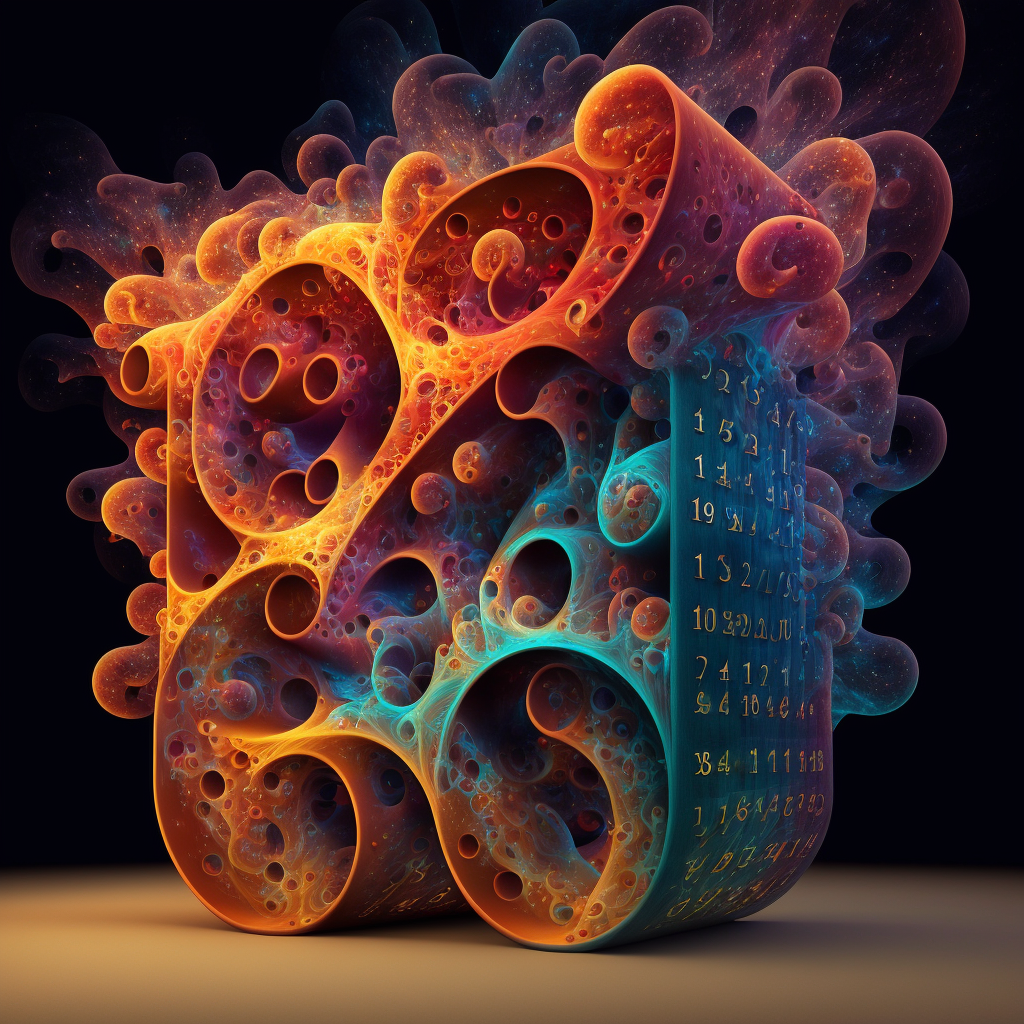
\includegraphics[scale=0.22]{./figs/chenle02_Stochastic_heat_equation.png}
  \end{center}
\end{frame}
\begin{frame}[fragile,t] % COMENTS
  \frametitle{Intermittency parabolic Anderson model Brownian motion...}
  \begin{center}
    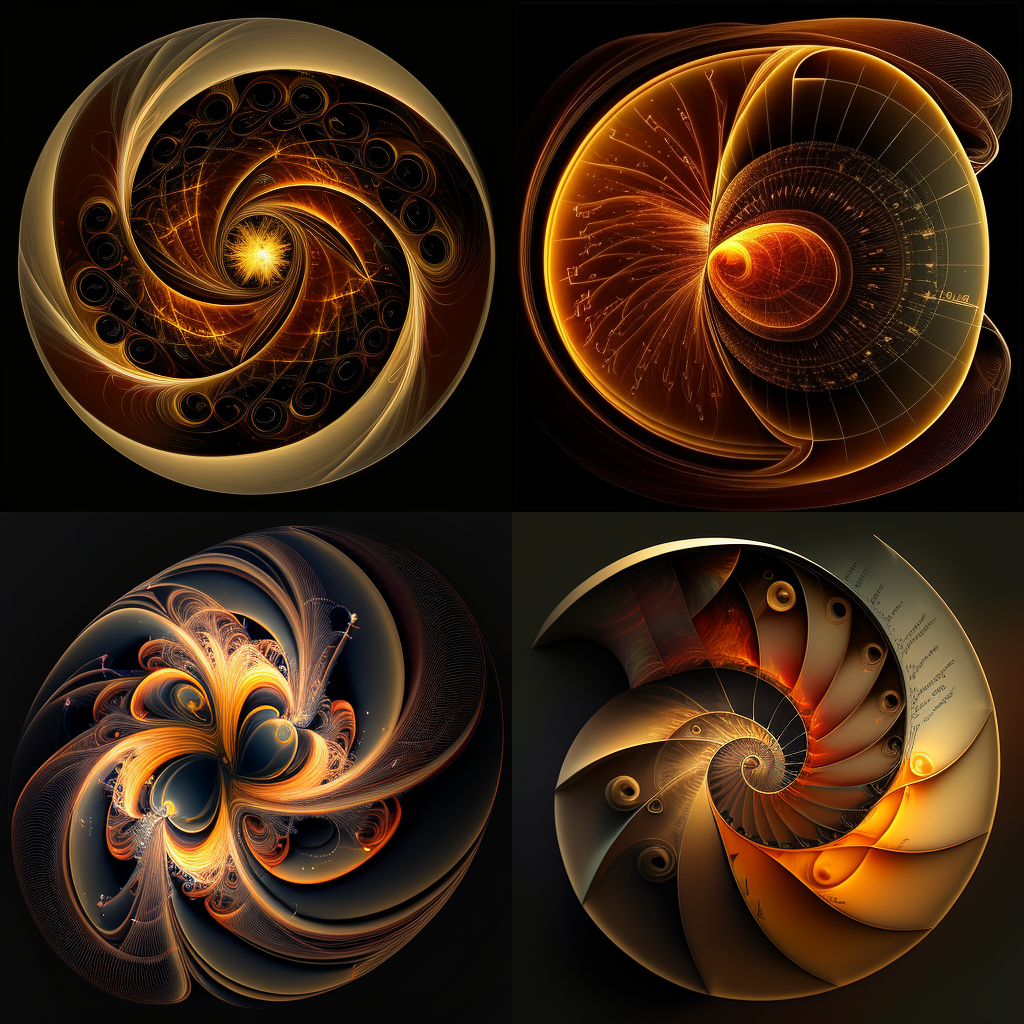
\includegraphics[scale=0.22]{./figs/chenle02_Intermittency_parabolic_Anderson_model_Brownian_motion.png}
  \end{center}
\end{frame}
\begin{frame}[fragile,t] % COMENTS
  \frametitle{A gitar placed in the sand storm in a desert show.png}
  \begin{center}
    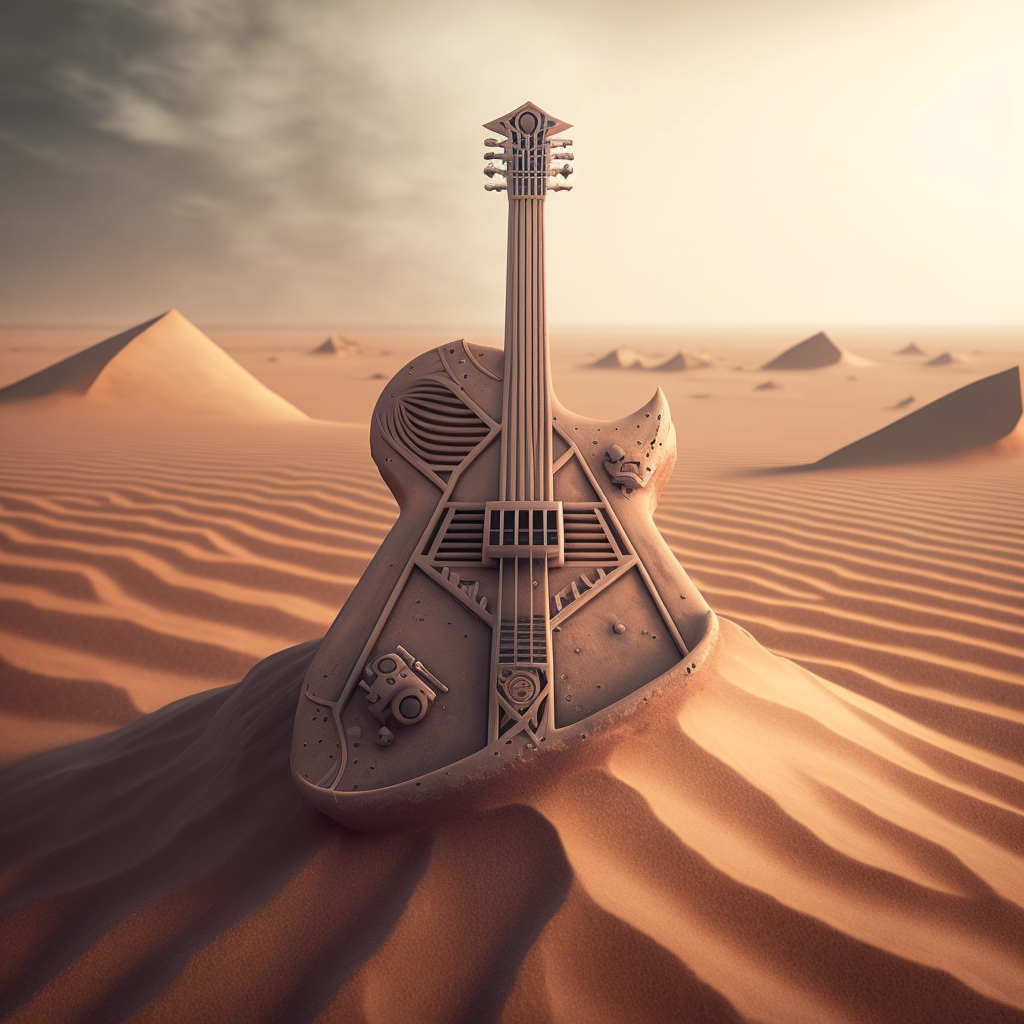
\includegraphics[scale=0.22]{./figs/chenle02_A_gitar_placed_in_the_sanddust_storm_in_a_desert_show.png}
  \end{center}
\end{frame}
\begin{frame}[fragile,t] % COMENTS
  \frametitle{Show rain drops on a small pond in a foggy raining day...}
  \begin{center}
    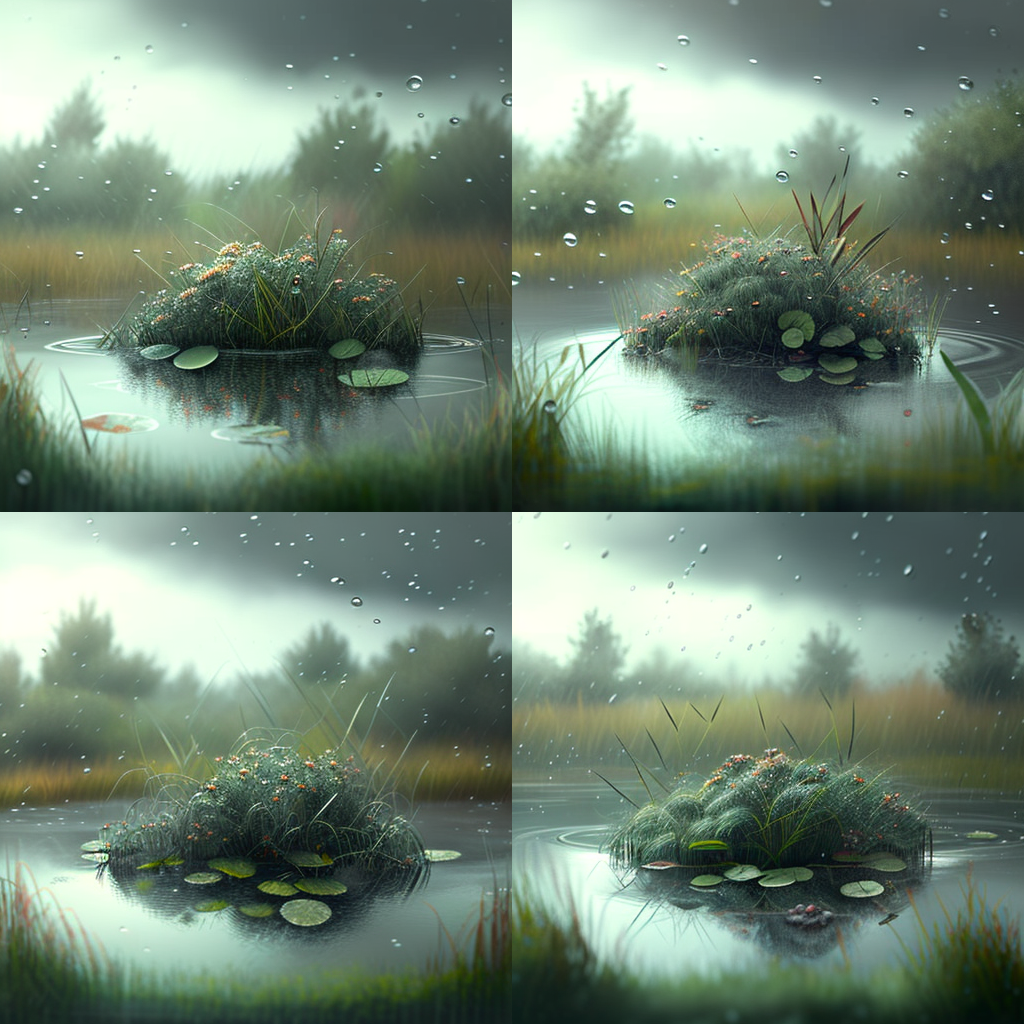
\includegraphics[scale=0.22]{./figs/chenle02_Show_rain_drops_on_a_small_pond_in_a_foggy_raining_day.png}
  \end{center}
\end{frame}
\begin{frame}[fragile,t] % COMENTS
  \frametitle{Lightning clouds dramatic light zigzag highly detailed...}
  \begin{center}
    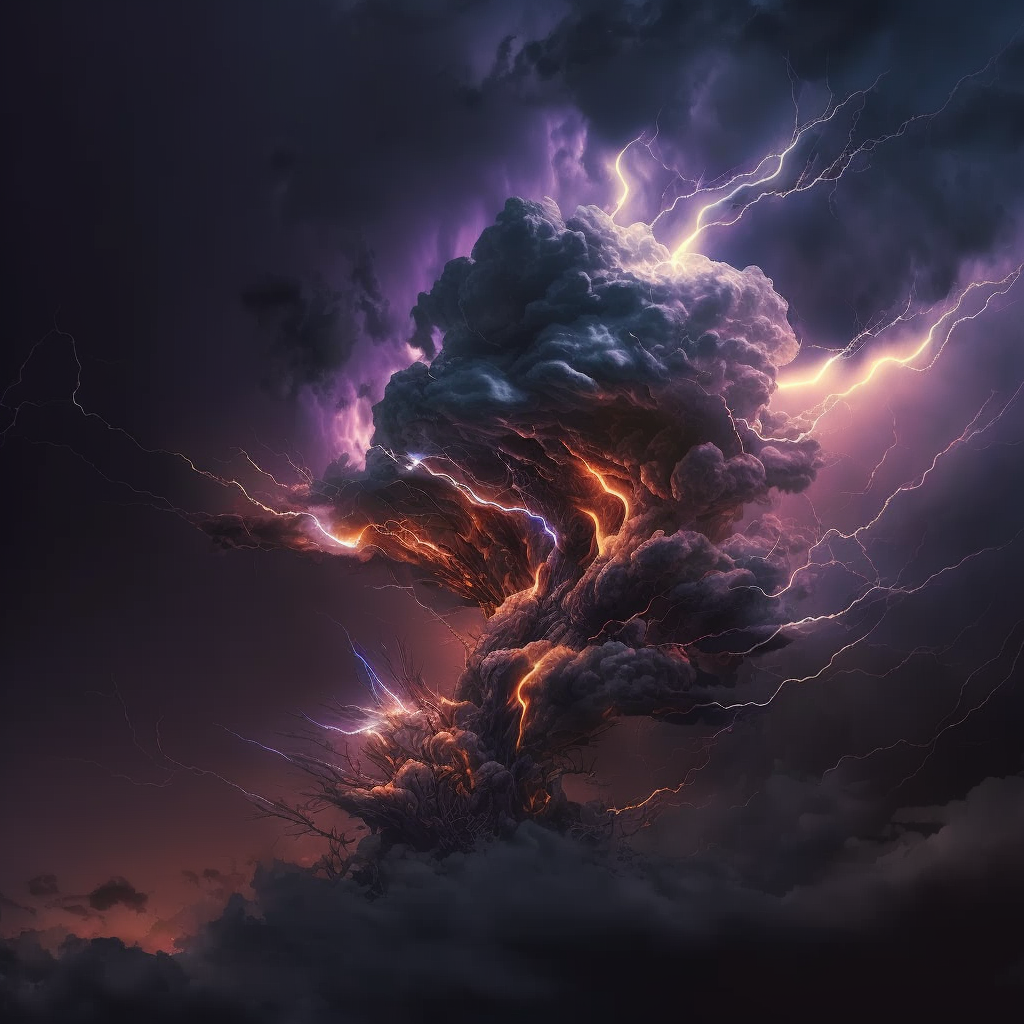
\includegraphics[scale=0.22]{./figs/chenle02_Lightningclouds_dramatic_light_zigzag_highly_detailed.png}
  \end{center}
\end{frame}
\begin{frame}[fragile,t] % COMENTS
  \frametitle{Mushrooms in clusters in a forest with sun shades...}
  \begin{center}
    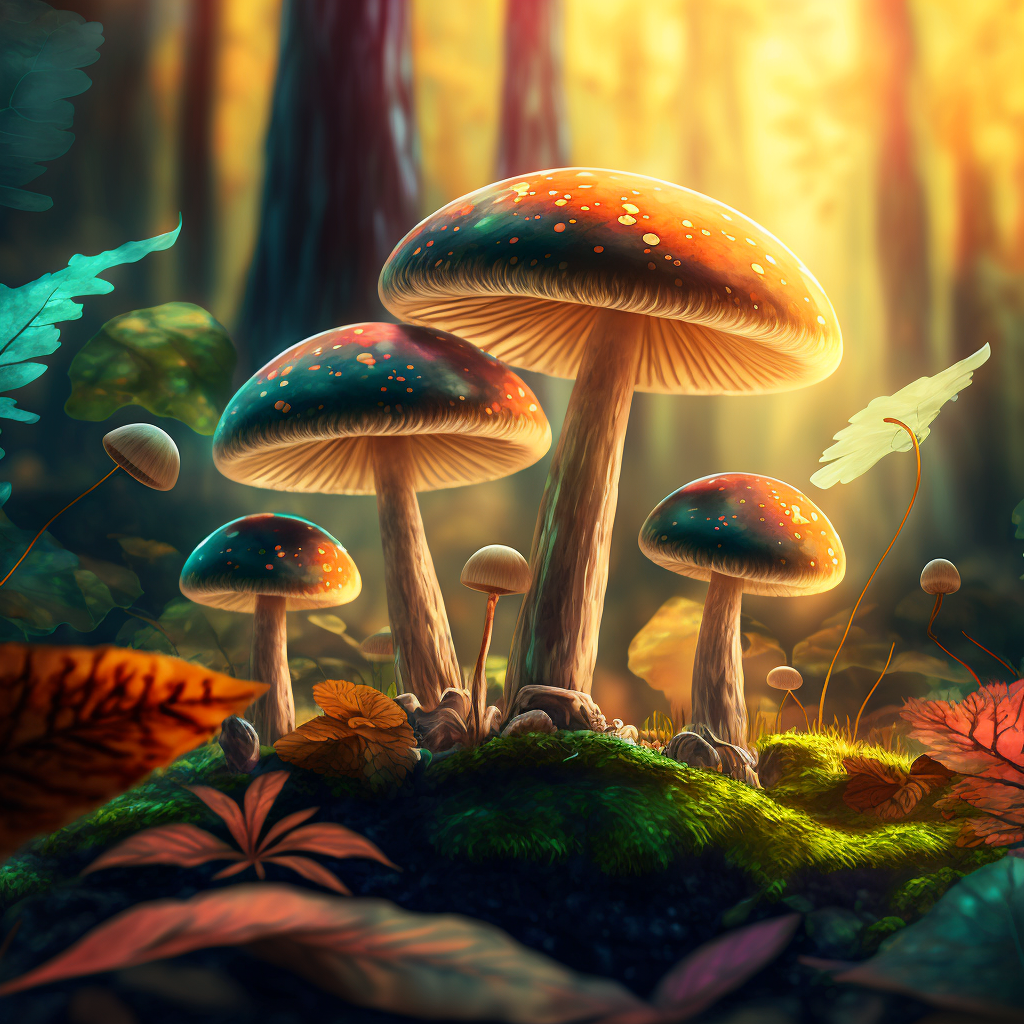
\includegraphics[scale=0.22]{./figs/chenle02_Mushrooms_in_clusters_in_a_forest_with_sun_shades_ultr.png}
  \end{center}
\end{frame}
\begin{frame}[fragile,t] % COMENTS
  \frametitle{Was it nuclear explosionor cosmic forces beyond comprehension...}
  \begin{center}
    
\includegraphics[scale=0.22]{./figs/chenle02_Was_it_nuclear_explosionor_cosmic_forces_beyond_comprehension.png}
  \end{center}
\end{frame}
\begin{frame}[fragile,t] % COMENTS
  \frametitle{Standing on the planet Mars looking at home the earth...}
  \begin{center}
    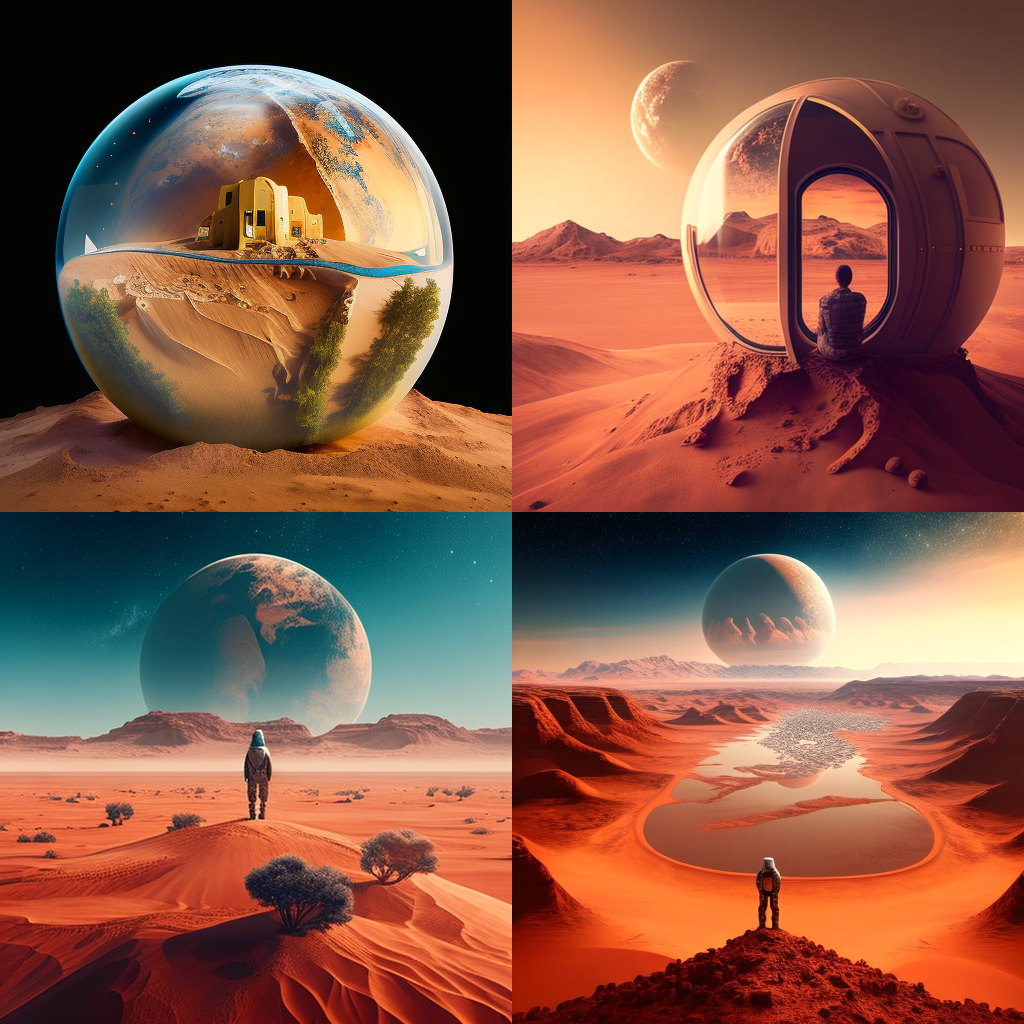
\includegraphics[scale=0.22]{./figs/chenle02_Standing_on_the_planet_Mars_looking_at_home_the_earth.png}
  \end{center}
\end{frame}
\begin{frame}[fragile,t] % COMENTS
  \frametitle{A homesick guy looking back to earth from Mars...}
  \begin{center}
    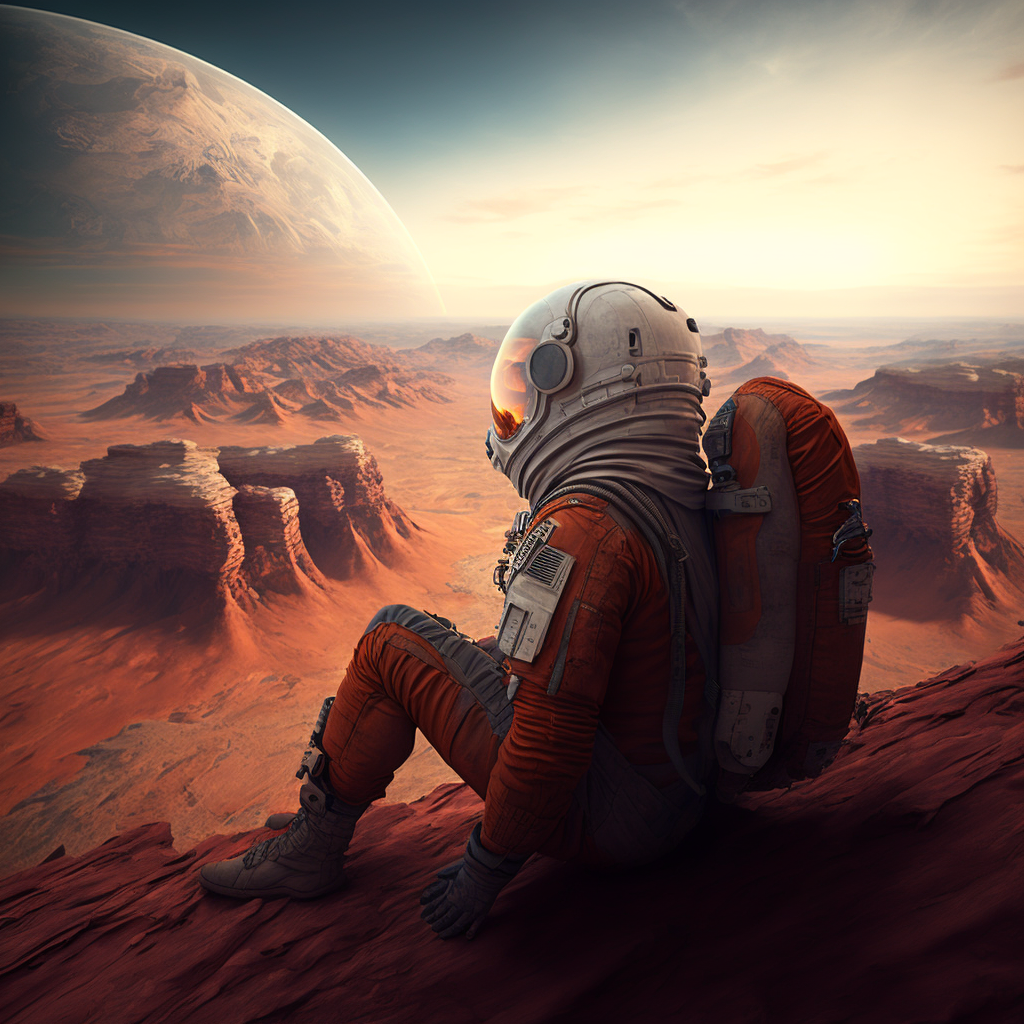
\includegraphics[scale=0.22]{./figs/chenle02_A_homesick_guy_looking_back_to_Earch_from_Mars_cinemar.png}
  \end{center}
\end{frame}
\begin{frame}[fragile,t] % COMENTS
  \frametitle{A person in front of the whole universe gallaxies...}
  \begin{center}
    
\includegraphics[scale=0.15]{./figs/chenle02_A_person_in_front_of_the_whole_universe_gallaxies.png}
  \end{center}
\end{frame}
\begin{frame}[fragile,t] % COMENTS
  \frametitle{Cosmic forces beyond comprehension...}
  \begin{center}
    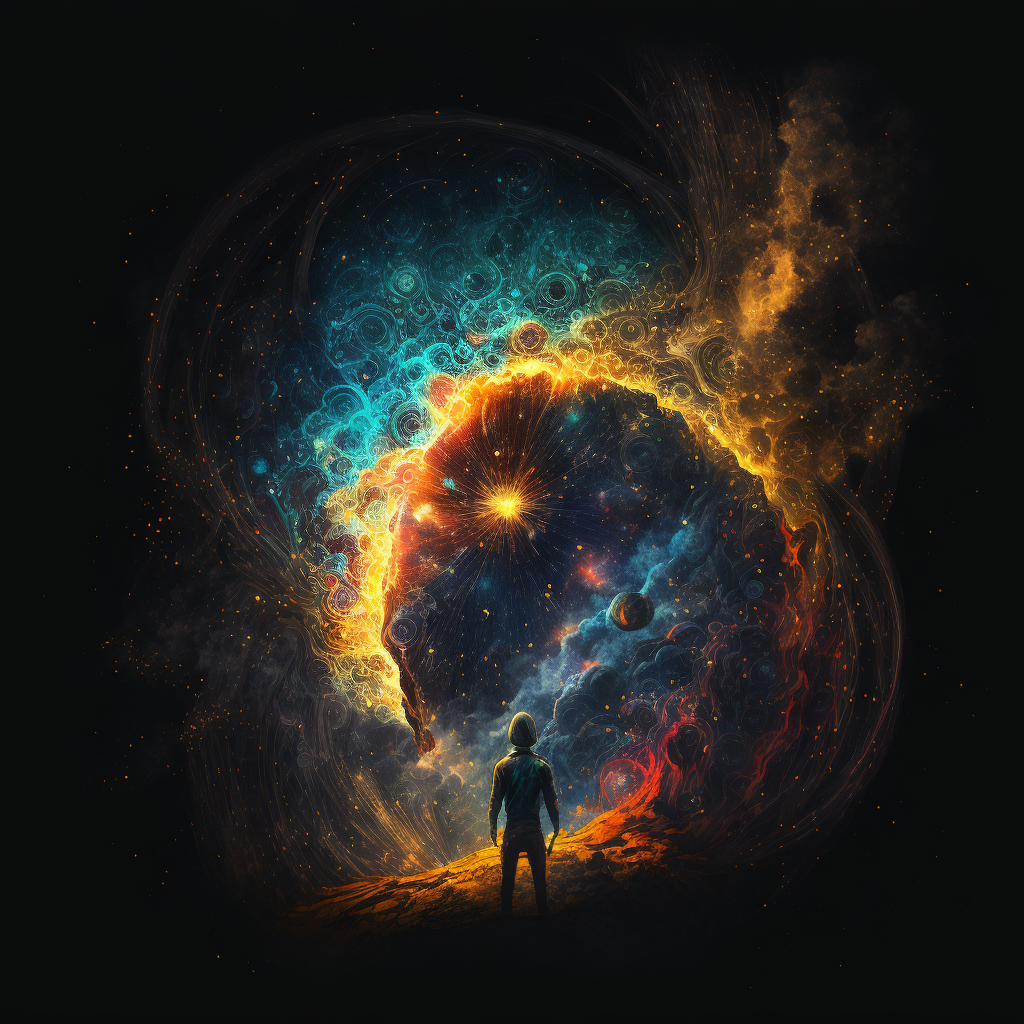
\includegraphics[scale=0.22]{./figs/chenle02_Cosmic_forces_beyond_comprehension.png}
  \end{center}
\end{frame}
\begin{frame}[fragile,t] % COMENTS
  \frametitle{Most famous mathematicians and physicist in the history...}
  \begin{center}
    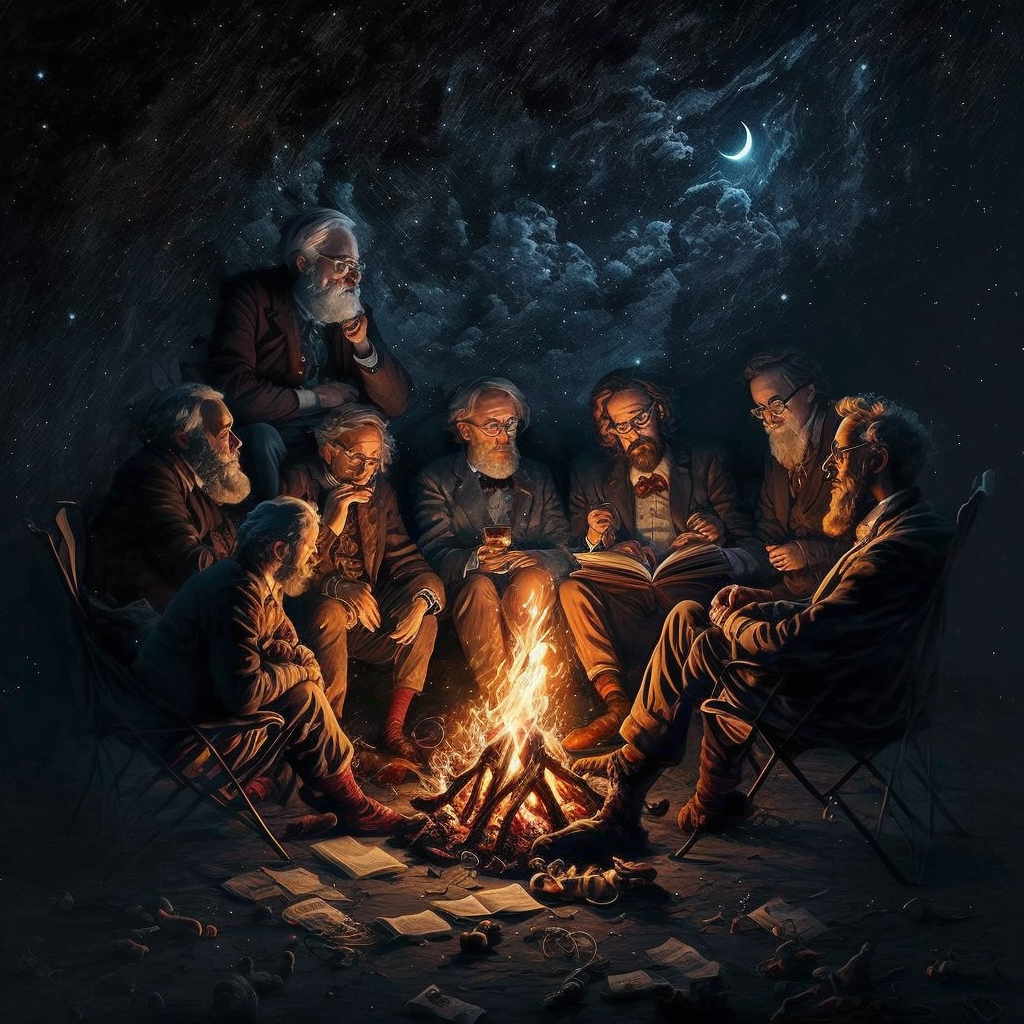
\includegraphics[scale=0.22]{./figs/chenle02_Most_famous_mathematicians_and_physists_in_the_history.png}
  \end{center}
\end{frame}
\section{Aknowledgement}
\begin{frame}[fragile,t] % COMENTS
  \begin{itemize}
    \item Le: {\small \it Write a sonnet for my math graduate students who
      attended my seminar talk about the using vim. git, github, and other
    tools to improve the workflow.}
    \vfill
    \item Chatgpt:
  \end{itemize}
   \begin{quotation}
      Oh, math graduate students, heed my call, \\
      For I bring tools to make your work sublime, \\
      With vim and git, you'll never fall, \\
      And on Github, your code will always shine.       \\ \bigskip

      Gone are the days of clunky text editors,         \\
      With vim's shortcuts, your fingers will dance,    \\
      No more worries of losing all your data,          \\
      For git's version control will give you a chance. \\ \bigskip

      And on Github, your code will come alive,         \\
      With collaboration at your fingertips,            \\
      Your workflow will be streamlined and thrive,     \\
      And your projects will be free from any slips.    \\ \bigskip

      So let us raise our glasses high,                 \\
      To vim, git, and Github, our allies.              \\
   \end{quotation}
\end{frame}
\begin{frame}<5->[fragile] % COMENTS
  \frametitle{Aknowledgement}

  \begin{center}
    \begin{minipage}{0.4 \textwidth}
      \Large
      \begin{itemize}
        \item Chatgpt
        \item Github Copilot
        \item Midjourney
      \end{itemize}
    \end{minipage}
  \end{center}


\end{frame}

\end{document}
